% 负责人：C / lanshuheng9-oss，对应 #5、#6、#7；跨重复结果由 B 补充。
\section{候选结构发现与可视化}
候选并不自动等于新结构。本节所有数值来自 2026 年 9 月 21 日 mask 修订后的正式运行，
完整命令、代码版本和结果表位于 \texttt{docs/results/}。

\subsection{候选发现与聚类}
我们用 WT rep1 中排除已知结构的 17 个训练背景窗口训练 32 维卷积自编码器，
4 个验证窗口选择轮次，3 个测试背景不参与训练或选轮次。逐窗口有效 mask 与上三角
mask 取交集后计算 loss，数据缺口的填零区域不参与训练和打分。模型在第 25 轮取得最佳
验证 masked MSE 0.022307。随后以 1 kb 步长扫描 4,641,652 bp 染色体，共得到
4,642 个 24 kb 窗口，并按重建误差前 1\% 保留 47 个候选。候选召回 21/344
个已知结构（6.1\%）；重建误差与接触强度的 Pearson 和 Spearman 相关分别为
0.828 和 0.765，因此高分明显受到接触密度影响，不能单独作为新结构证据。

候选、已知参考和 200 个固定种子随机背景使用同一编码器与标准化变换；背景从 1,075
个不与任何已知结构重叠的合格位置中抽取，实际重叠数为 0。标准化后保留
10 个白化 PCA 分量，再用 DBSCAN（\texttt{eps=3.0}，
\texttt{min\_samples=5}）聚类。相互重叠的候选窗口先合并，47 个窗口实际只有
10 个独立位置。唯一的非噪声簇包含 297 个已知参考成员；其中 9 个候选来自
4 个独立区域，4 个还直接与已知结构重叠。其余 38 个候选为 DBSCAN 噪声。

本组约定疑似新簇必须同时包含至少 5 个独立候选位置、没有已知参考成员，且候选区间
均不与已知结构重叠；DBSCAN 的 $-1$ 噪声不算簇。本次没有任何簇满足规则，因此不
宣称发现新结构，留待跨重复任务检查全部候选。作为表征检查，306 个无歧义已知参考
位置按完整窗口的空间重叠连通关系分成 60 组，再做 5 折平衡逻辑回归；实测跨折重叠
对数为 0，balanced accuracy 为 0.518，多数类 balanced accuracy 为 0.333，说明
隐向量含有有限类别信息，但不足以替代正式分类器。

\begin{figure}[htbp]
  \centering
  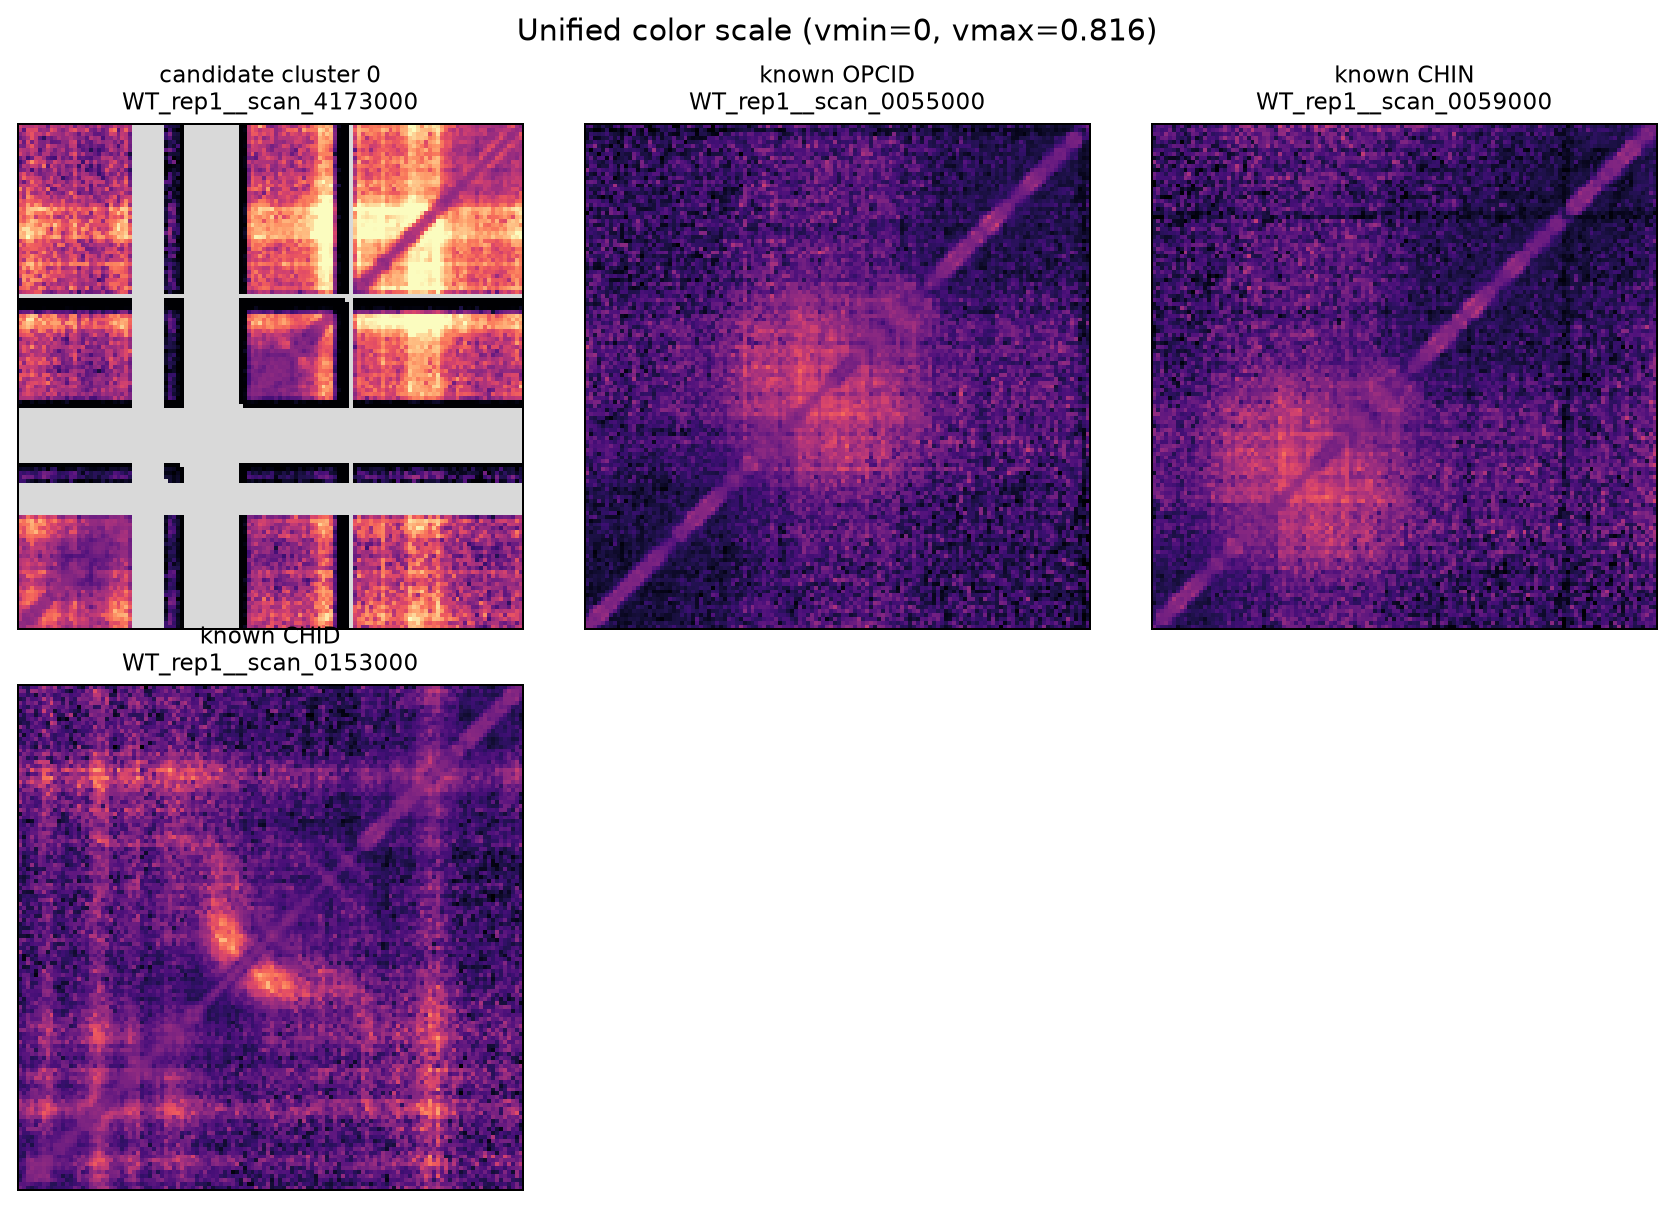
\includegraphics[width=0.92\linewidth]{../results/clustering/cluster_representatives.png}
  \caption{候选簇代表与三类已知结构参考。所有热图统一使用 0--0.816 色标，灰色为无效像素。}
\end{figure}

\subsection{全基因组多轨道图}
轨道信号复用 100 bp 共享缓存：上三角非对角接触累加到两个端点，对角接触只计一次，
再按每个样本的总接触量缩放至每百万，先归一化两个重复再取条件均值。图上使用平方根
显示压缩动态范围，原始保存数组仍是线性归一化信号。

WT、$\Delta stpA$ 和 $\Delta hns\Delta stpA$ 三条件共六个真实重复被绘制为四面板图：
重复曲线及全基因组中位数灰线、条件均值、基因轨道和 CHIN/OPCID 轨道。全基因组按
10 kb 输出 465 张，末图正确覆盖 $[4,640,000,4,641,652)$；最后不足 100 bp 的无效
bin 留白，没有画成假性零值。首图、末图和 4 张代表图均已人工检查，完整图集位于本地
\texttt{outputs/tracks/all/}，可提交的运行记录和代表图位于
\texttt{docs/results/tracks/}。

不同条件下的局部趋势并不一致：$[1{,}210{,}000,1{,}220{,}000)$ 和
$[2{,}480{,}000,2{,}490{,}000)$ 中双突变条件在多数位置高于其他两组，
$[3{,}800{,}000,3{,}810{,}000)$ 则主要表现为 $\Delta stpA$ 信号较高。这些图用于展示
轨道的实际读法与局部差异，不把单个区间的曲线高低当作全基因组显著性结论。

\begin{figure}[htbp]
  \centering
  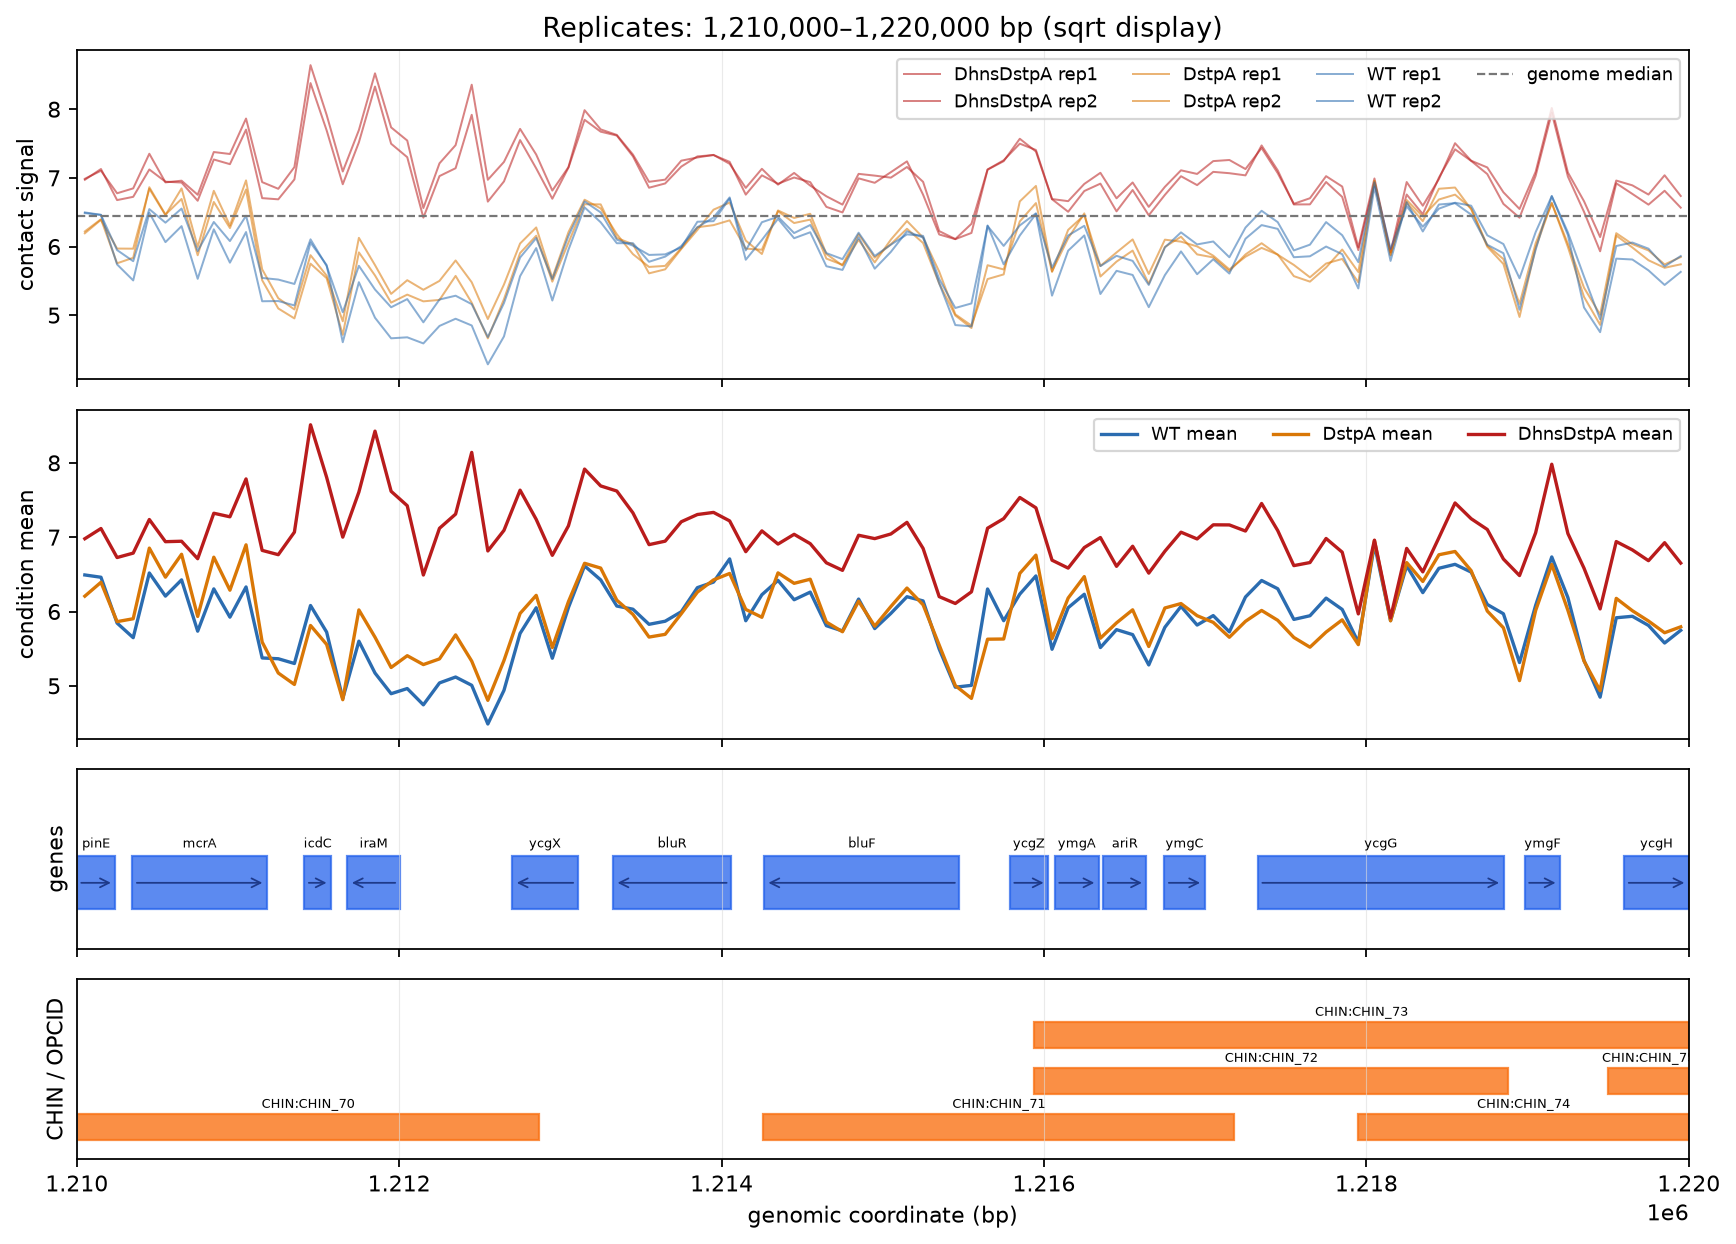
\includegraphics[width=0.96\linewidth]{../results/tracks/tracks_1210000_1220000.png}
  \caption{$[1{,}210{,}000,1{,}220{,}000)$ 的三条件轨道。每个重复先独立归一化，条件均值在线性尺度上计算后再开平方显示。}
\end{figure}

\begin{figure}[htbp]
  \centering
  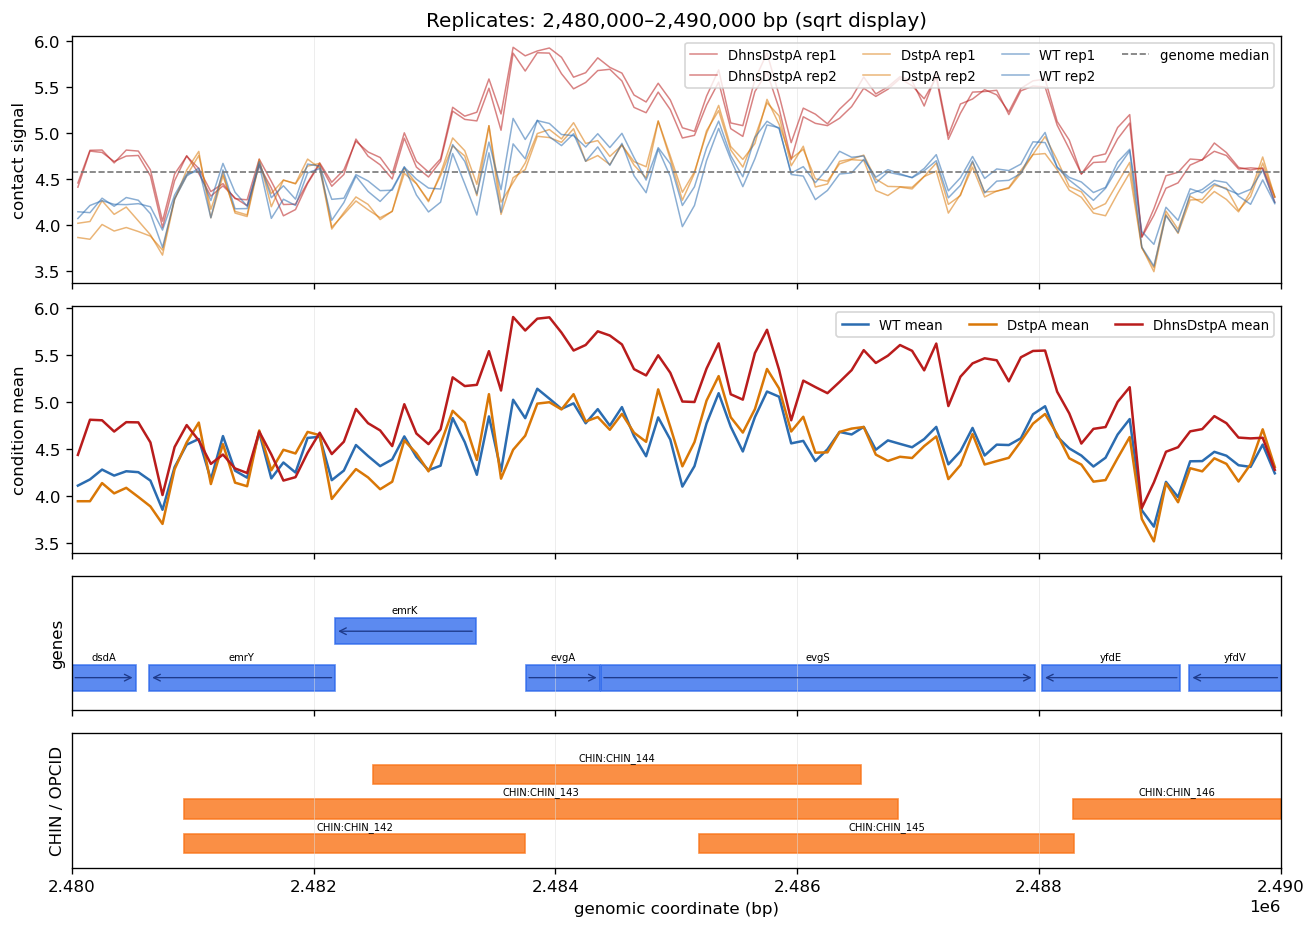
\includegraphics[width=0.96\linewidth]{../results/tracks/tracks_2480000_2490000.png}
  \caption{$[2{,}480{,}000,2{,}490{,}000)$ 的三条件轨道。图中同时保留重复曲线、条件均值、基因与已知结构坐标。}
\end{figure}

\begin{figure}[htbp]
  \centering
  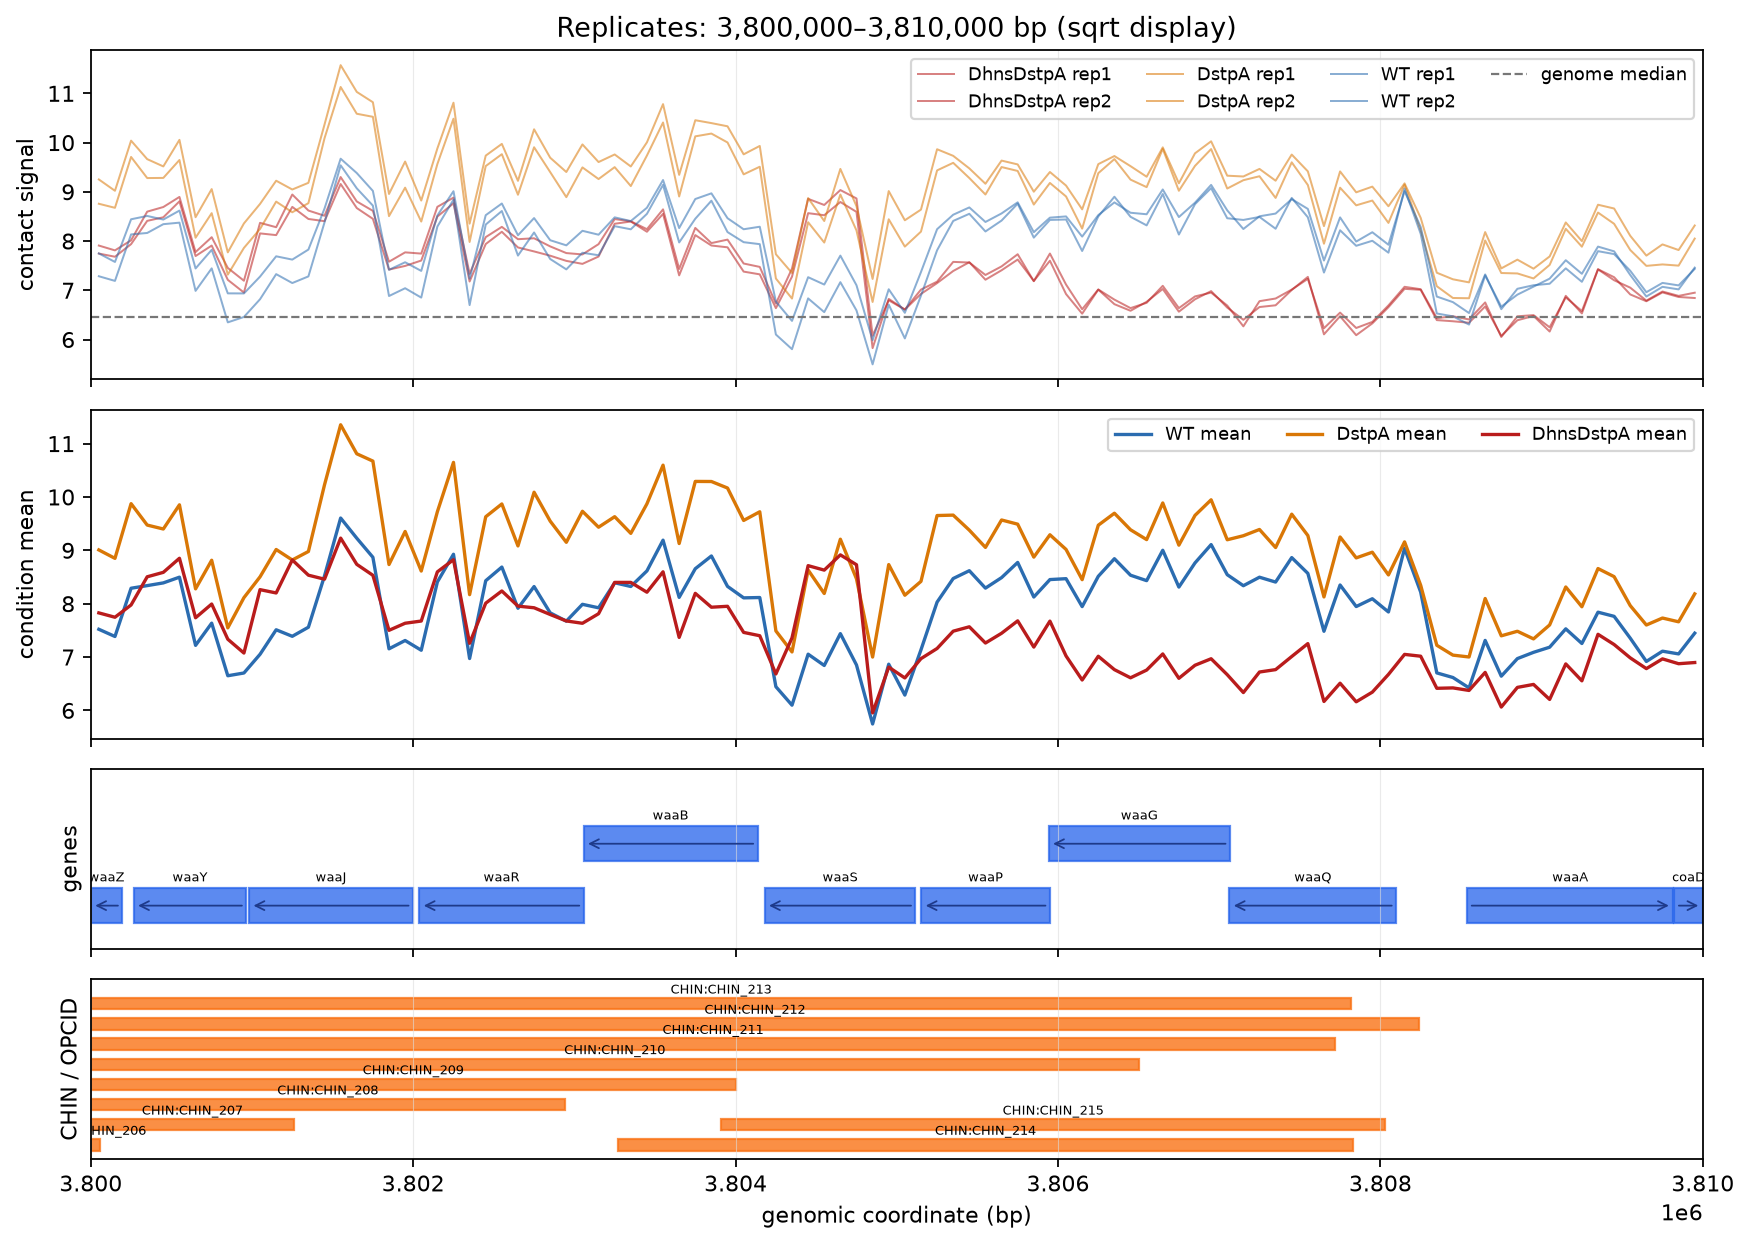
\includegraphics[width=0.96\linewidth]{../results/tracks/tracks_3800000_3810000.png}
  \caption{$[3{,}800{,}000,3{,}810{,}000)$ 的三条件轨道。本区间与前两例呈现不同的条件顺序，说明不应使用单个代表区间概括全基因组。}
\end{figure}
